\documentclass{beamer}
\usepackage{polski}
\usepackage[utf8]{inputenc}
\usepackage{pgf-pie}
\usepackage{graphicx}  % Do obsługi obrazów
\usepackage{natbib}    % Do obsługi bibliografii
\usepackage{pgfplots}
\pgfplotsset{compat=1.17}
\title{PyPou}
\author{Jan Rolka, Paweł Rycerz, Bartłomiej Wolny, Emanuel Sujeta, Patrick Bajorski, Jakub Łabuz}
\institute{AGH}
\date{2023}

\begin{document}

\frame{\titlepage}

\begin{frame}{PyPou - Gra inspirowana Pou}
Celem projektu jest stworzenie gry komputerowej \textbf{PyPou} w oparciu o bibliotekę \textit{Pygame}\cite{coding_with_russ_kanal_nodate}, która będzie podobna do popularnej gry mobilnej \textit{Pou}. Gra będzie polegać na opiece nad wirtualnym zwierzakiem, rozwijaniu go i spełnianiu jego wszelakich potrzeb. Najważniejszą częścią gry będą wszelkiego rodzaju minigry, dzięki którym podniesiemy poziom zadowolenia naszego podopiecznego oraz zarobimy nieco specjalnej waluty.
\begin{figure}[h]
  \centering
  
\includegraphics[width=0.3\textwidth]{grafiki/PyPou.png}
  \caption{To jest nasz PyPou}
\end{figure}
\end{frame}

\begin{frame}{Minigry}
    Gra zawiera szereg minigier takich jak:
    \begin{itemize}
        \item Flappy PyPou
        \item TetriPou
        \item DinoPou
        \item Icy Tower
        \item PingPou
        \item PySaga
    \end{itemize}
\end{frame}

\begin{frame}{Interfejs}
    Głowny interfejs naszej gry, będący mieszakniem PyPou prezentuje się następująco:
    \begin{figure}
        \centering
        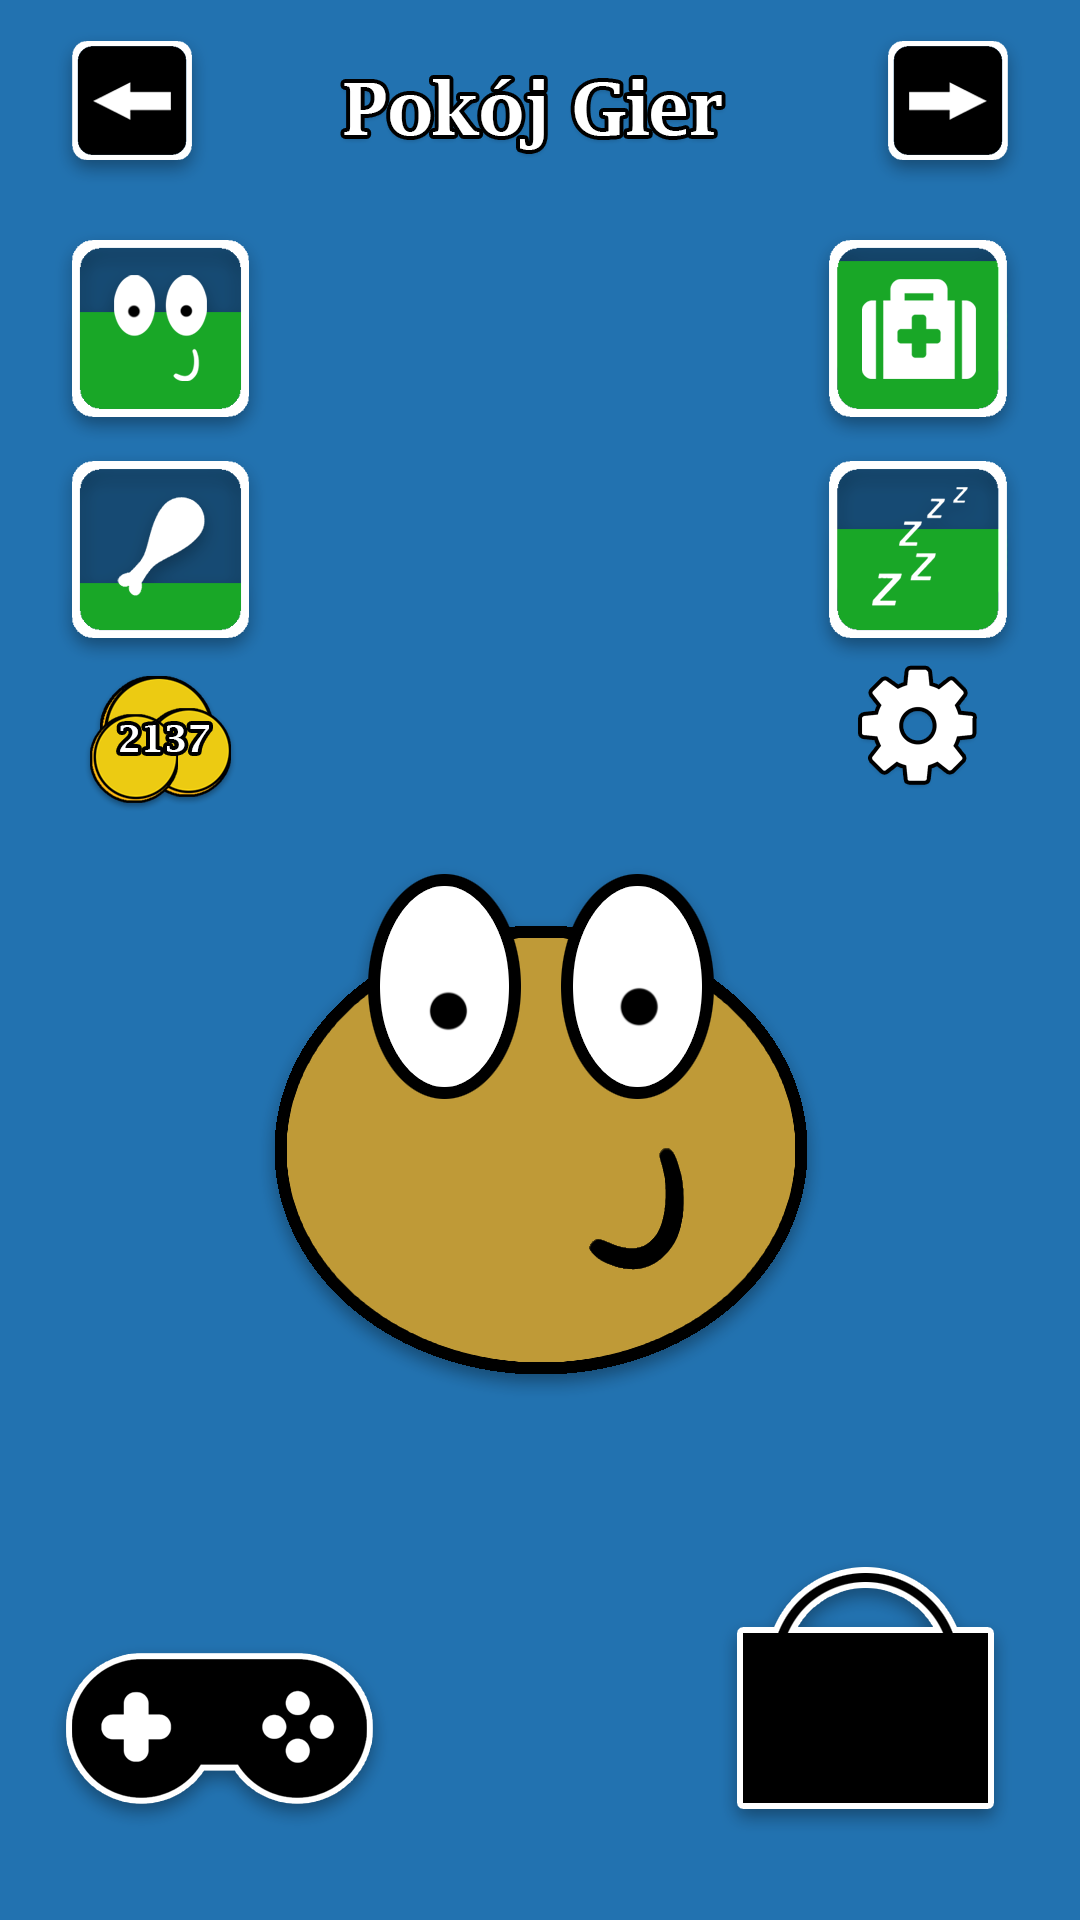
\includegraphics[width=0.3\textwidth]{grafiki/prototypUI3.png}
        \caption{Interfejs przy rozpoczęciu gry}
        \label{fig:UI1}
    \end{figure}
\end{frame}

\begin{frame}{Interfejs po modyfikacjach jakich może dokonać gracz}
    Gracz wraz z progresem może coraz bardziej modyfikować PyPou oraz jego otoczenie
    \begin{figure}
        \centering
        
\includegraphics[width=0.3\textwidth]{grafiki/prototypUI_kuchnia1.png}
        \caption{Interfejs po modyfikacjach}
        \label{fig:UI2}
    \end{figure}
\end{frame}

\begin{frame}{Informacje na ekranie}
    \begin{figure}%
    \centering
    \subfloat{{
\includegraphics[width=0.3\textwidth]{grafiki/ikonka zadowolenia.png} }}%
    \qquad
    \subfloat{{
\includegraphics[width=0.3\textwidth]{grafiki/ikonka zdrowia.png} }}%
    \qquad
    \subfloat{{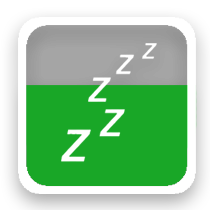
\includegraphics[width=0.3\textwidth]{grafiki/ikonka zmeczenia.png} }}%
    \qquad
    \subfloat{{
\includegraphics[width=0.3\textwidth]{grafiki/ikonka jedzenia.png} }}%
    \caption{Ikonki stanu naszego PyPou}%
    \label{fig:example}%
    \end{figure}
\end{frame}

\begin{frame}
\frametitle{Analiza wyników ankiety}
Oto jak rozłożył się udział jezyków programowania:
\begin{figure}[h]
  \centering
  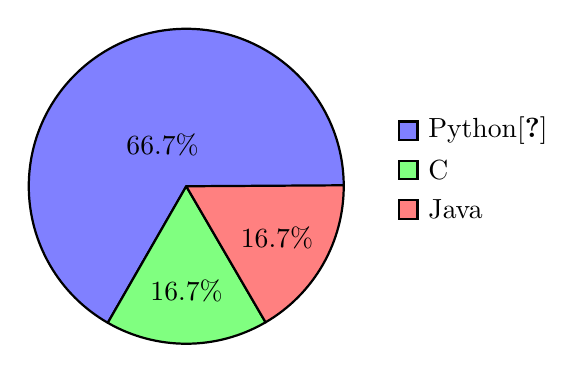
\begin{tikzpicture}
    \pie[text=legend, color={blue!50, green!50, red!50}, radius=2]
      {66.7/Python\cite{noauthor_oficjalna_nodate}, 16.7/C, 16.7/Java}
  \end{tikzpicture}
  \caption{Procentowy udział j\cite{noauthor_oficjalna_nodate}ęzyków programowania.}
  \label{fig:wykres_kolowy}
\end{figure}
Z tego powodu zdecydowaliśmy się na stworzenie gry w języku python.
Gra polega na dużej ilości minigier, co daje sporo frajdy, szczególnie docelowej grupie odbiorców, czyli dzieciom.
\end{frame}

\begin{frame}{Motywacja dla projektu}
Motywacją do powstania naszego projektu była przede wszystkim chęć sprawdzenia własnych zdolności programistycznych.
Chcieliśmy się również jak najwięcej nauczyć\cite{david_j_malan_kurs_nodate}\cite{kanal_o_wszystkim_kurs_nodate} i zdobyć cenne, rozwijające doświadczenie.
Oczywiście zależało nam też na dobrej zabawie i rozwijaniu kreatywności oraz umiejętności pracy zespołowej.
Projekt ten jest również naszym pierwszym zetknięciem z szeroko pojętym światem tworzenia gier wideo, który obecnie jest jednym z najbogatszych i najszybciej rozwijających się sektorów informatyki.

\end{frame}

\begin{frame}{Ciekawy wykres}
A o to wykres przedstawiający dynamikę rozwoju światowego rynku gier.
Biorąc pod uwagę, że prawdopodobnym jest, że w przyszłości będziemy pracować w tym sektorze, już dziś warto nabierać doświadczenia.
Pierwszym małym krokiem jest omawiany projekt.

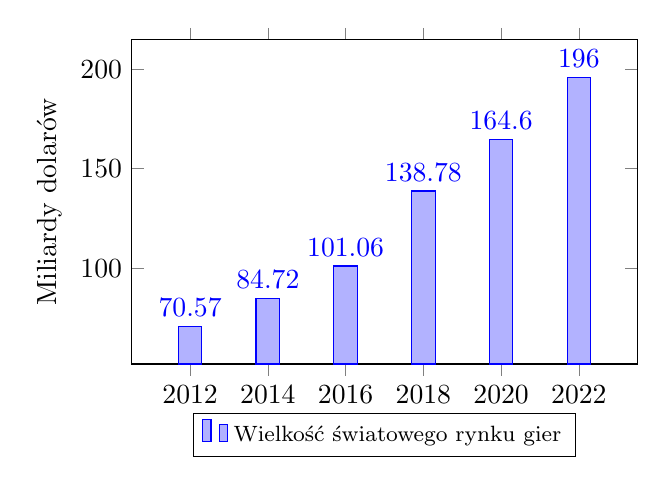
\begin{tikzpicture}
\begin{axis}[
    width=8cm, % Szerokość wykresu
    height=5.7cm, % Wysokość wykresu
    ybar,
    bar width=0.3cm, % Szerokość słupków
    enlargelimits=0.15,
    legend style={at={(0.5,-0.15)},
    anchor=north,legend columns=-1},
    ylabel={Miliardy dolarów},
    xtick=data,
    xticklabels={2012,2014,2016,2018,2020,2022}, % Etykiety lat
    nodes near coords,
    nodes near coords align={vertical},
    every axis title/.style={font=\small}, % Zmniejszenie czcionki tytułu osi Y
    every axis legend/.append style={font=\footnotesize}, % Zmniejszenie czcionki legendy
    ]
\addplot coordinates {(2012,70.57) (2014,84.72) (2016,101.06) (2018,138.78) (2020,164.60) (2022,196.00)}; % Dane 1
\legend{Wielkość światowego rynku gier} % Legenda
\end{axis}
\end{tikzpicture}

\end{frame}

\begin{frame}{Bibliografia z odnośnikami}
    % Sekcja bibliografii
    \bibliographystyle{plain}
    \bibliography{bibliografia.bib}
\end{frame}

\end{document}
